% exercise sheet with header on every page for math or close subjects
\documentclass[12pt]{article}
\usepackage[utf8]{inputenc} 
\usepackage{latexsym} 
\usepackage{multicol}
\usepackage{fancyhdr}
\usepackage{amsfonts} 
\usepackage{amsmath}
\usepackage{amssymb}
\usepackage{enumerate}
\usepackage{listings}
\usepackage{graphicx}
\usepackage{pdfpages}

% Shortcuts for bb, frak and cal letters
\newcommand{\E}{\mathbb{E}}
\newcommand{\V}{\mathbb{V}}
\renewcommand{\P}{\mathbb{P}}
\newcommand{\N}{\mathbb{N}}
\newcommand{\R}{\mathbb{R}}
\newcommand{\C}{\mathbb{C}}
\newcommand{\Z}{\mathbb{Z}}
\newcommand{\Pfrak}{\mathfrak{P}}
\newcommand{\Pfrac}{\mathfrak{P}}
\newcommand{\Bfrac}{\mathfrak{P}}
\newcommand{\Bfrak}{\mathfrak{B}}
\newcommand{\Fcal}{\mathcal{F}}
\newcommand{\Ycal}{\mathcal{Y}}
\newcommand{\Bcal}{\mathcal{B}}
\newcommand{\Acal}{\mathcal{A}}

% formating
\topmargin -1.5cm 
\textheight 24cm
\textwidth 16.0 cm 
\oddsidemargin -0.1cm

% Fancy Header on every Page
\pagestyle{fancy}
\lhead{\textbf{Programmierung for Engineers - Exercise 1}}
\rhead{Daniel Schäfer (2549458)\\ Dominik Weber}
\renewcommand{\headrulewidth}{1.2pt}
\setlength{\headheight}{110pt} 

\begin{document}
\pagenumbering{gobble}
\lstset{language=C++}

\section{ Erste Schritte mit dem Arduino Mega}
\begin{enumerate}
    \item 
        ein weiteres \verb!delay! unter der Zeile \verb!digitalWrite(led , LOW);! einfuegen. Siehe zB code aus Aufgabe 1.2 a)
        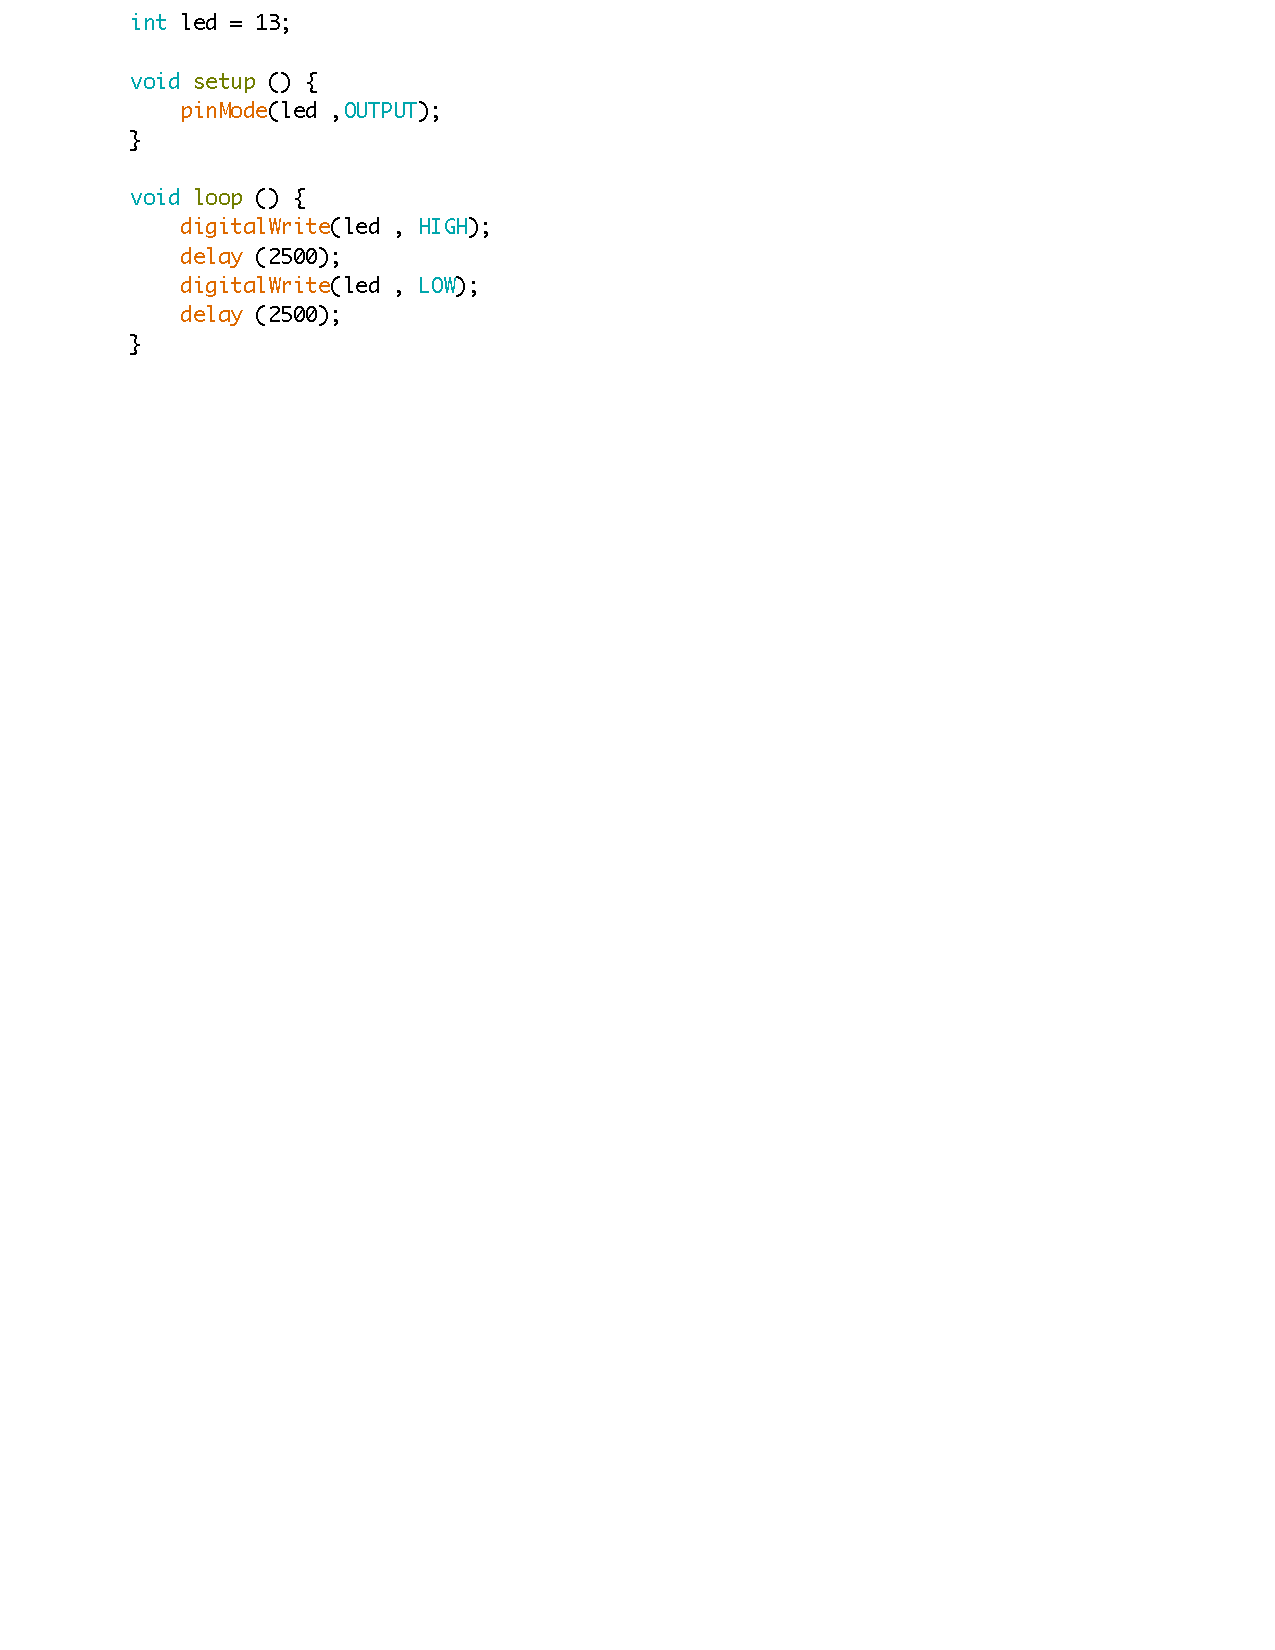
\includepdf[pages=-]{../aufgabe11/aufgabe11.pdf}
    \item
        \begin{enumerate}[a)]
            \item 
                see code on the next page:\\
                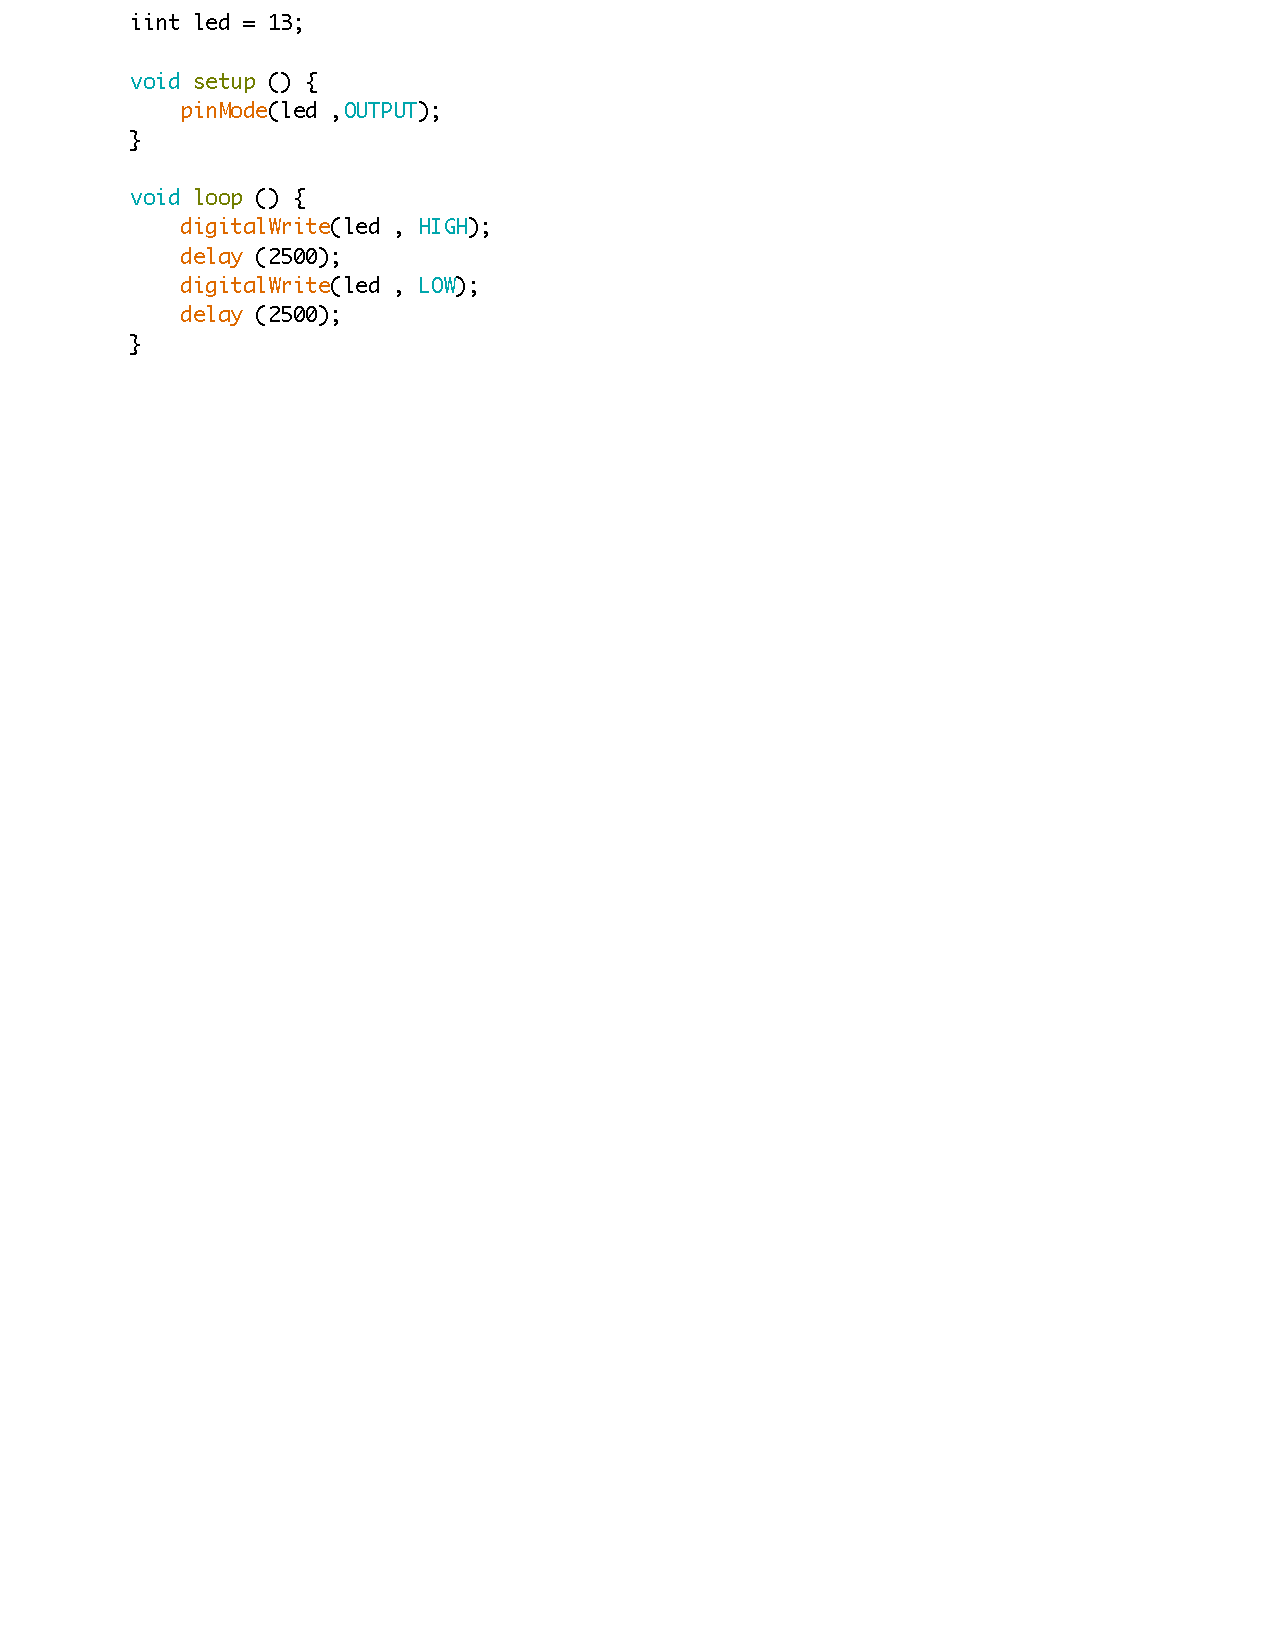
\includepdf[pages=-]{../aufgabe12a/aufgabe12a.pdf}

            \item
                see code on the next page:\\
                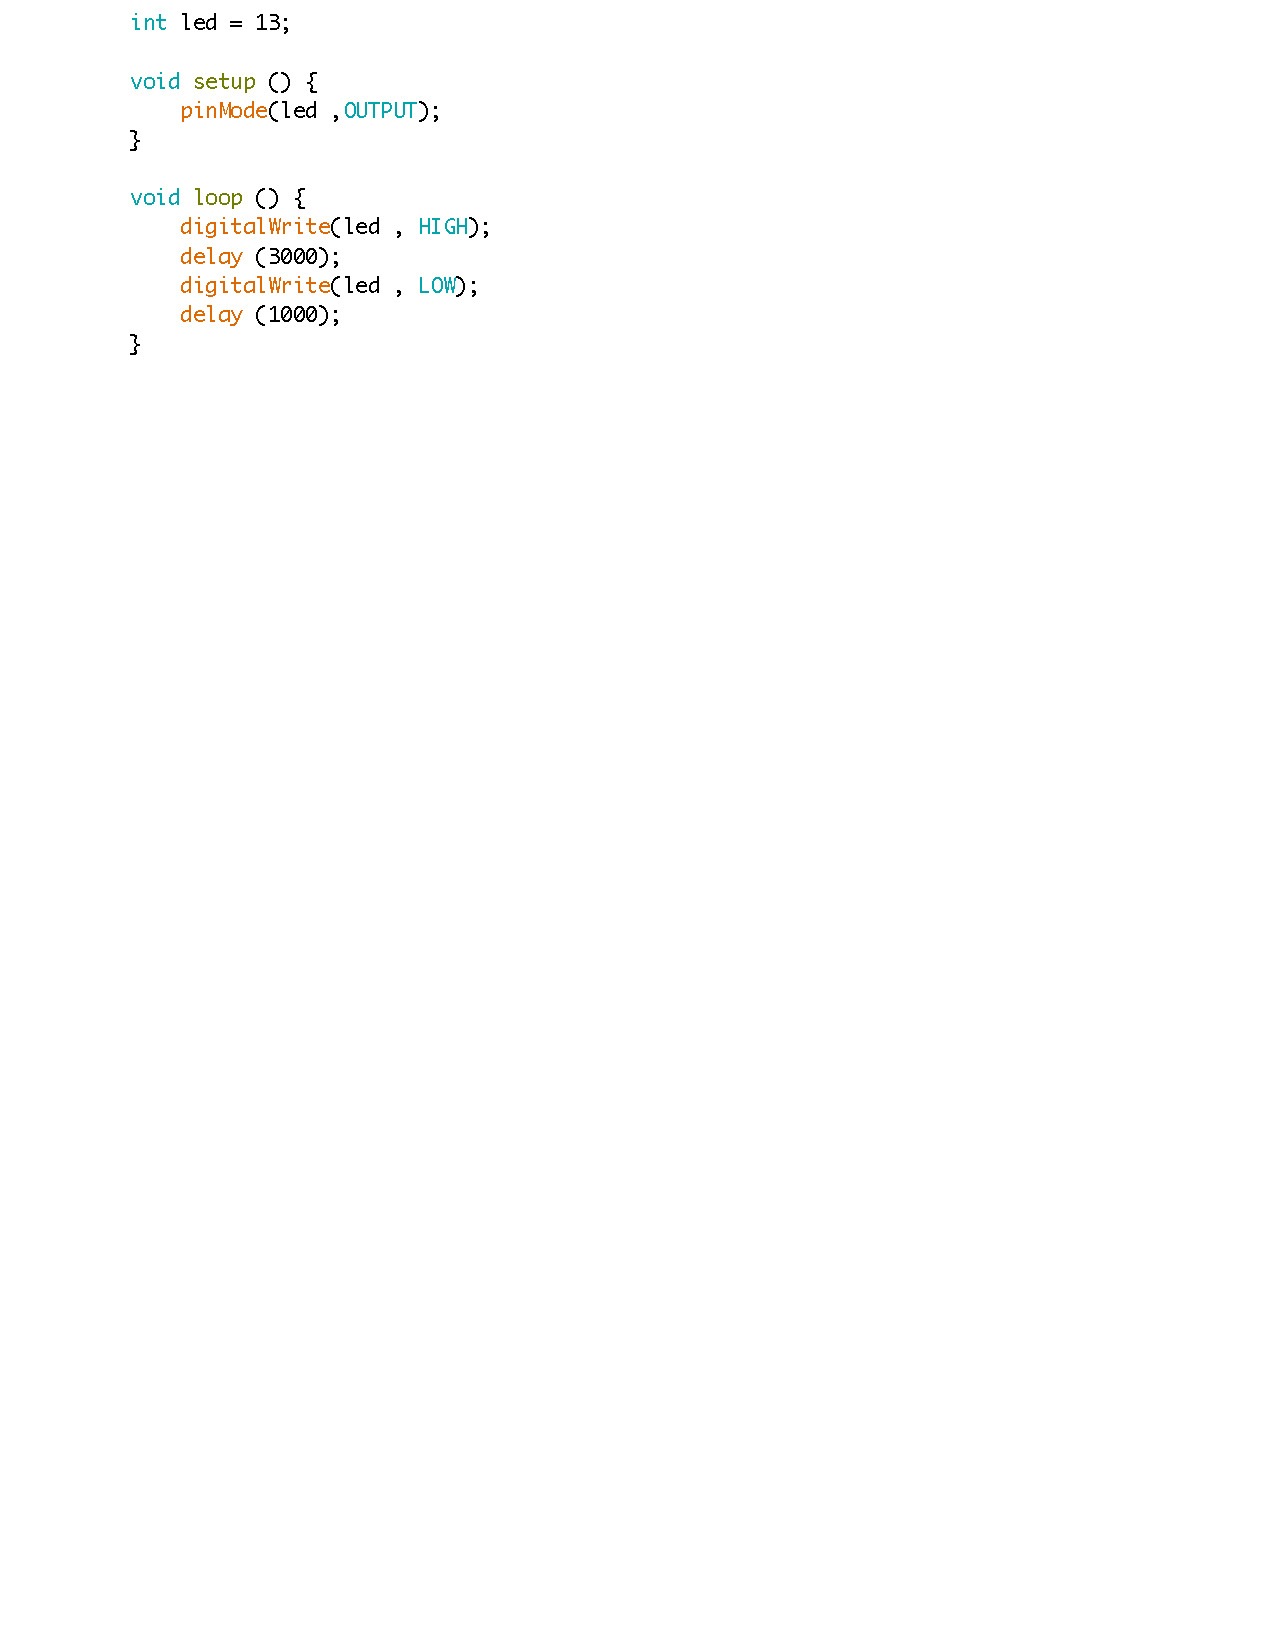
\includepdf[pages=-]{../aufgabe12b/aufgabe12b.pdf}

            \item
                see code on the next page:\\
                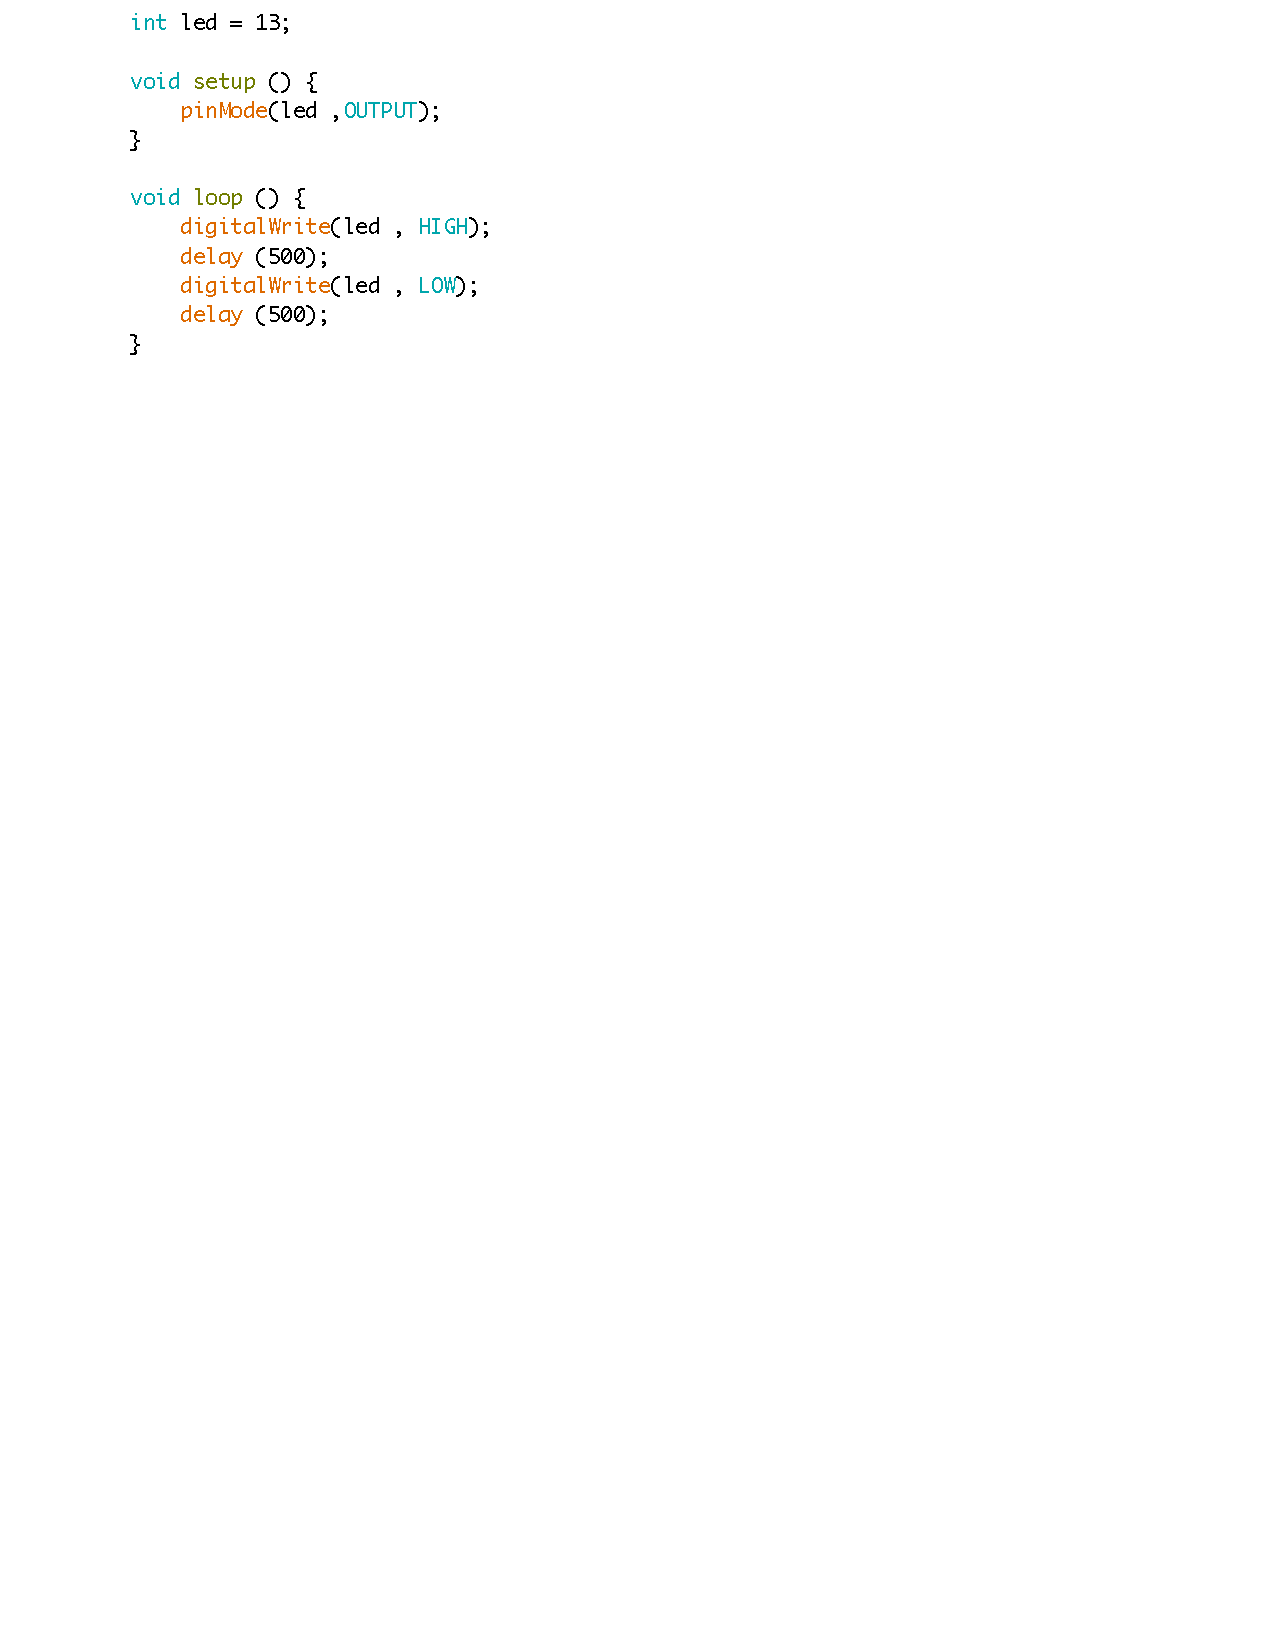
\includepdf[pages=-]{../aufgabe12c/aufgabe12c.pdf}
                
        \end{enumerate}
\end{enumerate}


    \newpage
\section{Morse}

\begin{enumerate}
    \item
        see code on the next page\\
        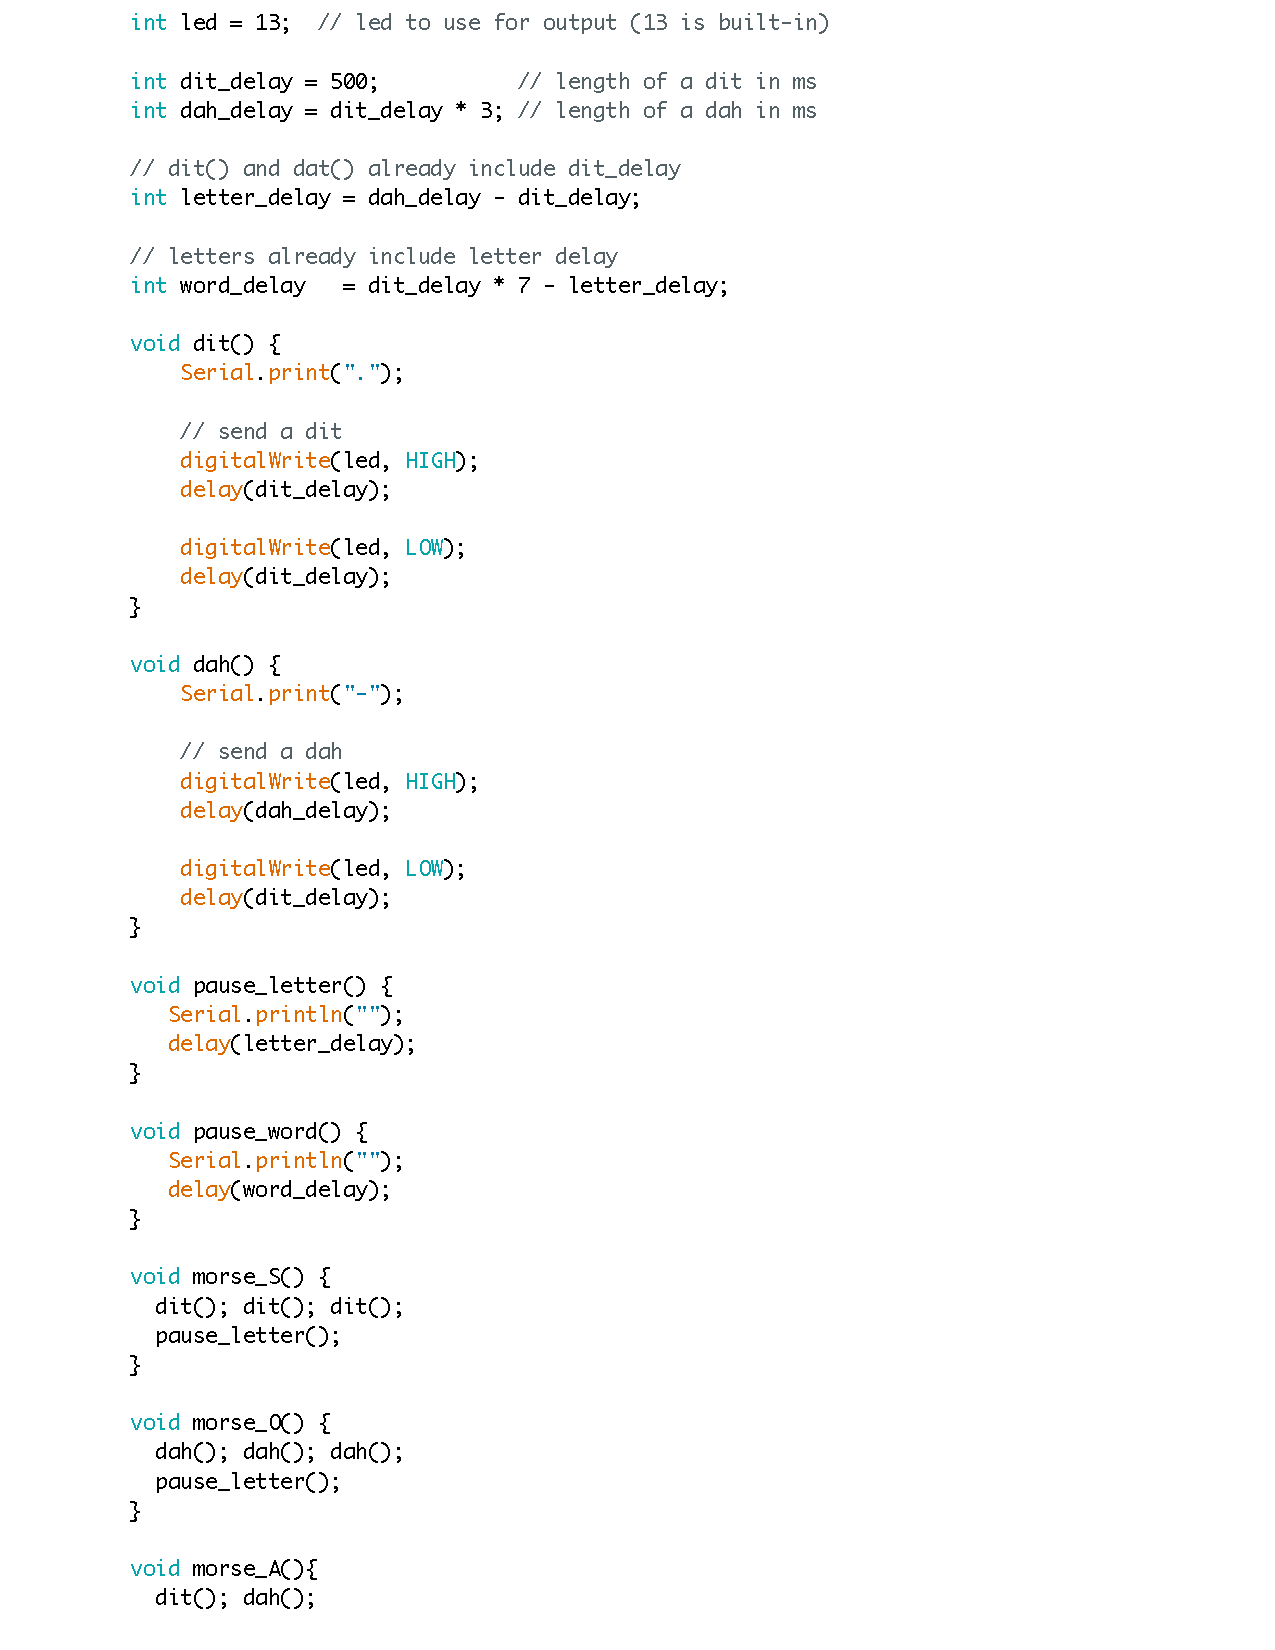
\includepdf[pages=-]{../aufgabe21/aufgabe21.pdf}

    \item
        with the used approach this would be very messy! Essentially you rewrite the approach by using an int argument called \verb!LED_id! to all functions called \verb!morse_A(int LED_id)!, \verb!morse_B(int LED_id)! and so on. Instead of calling \verb! dit()! and \verb!dah()! we would call \verb!dit(int LED_id)! and \verb!dah(int LED_id)!. The functions would look like this:\\

        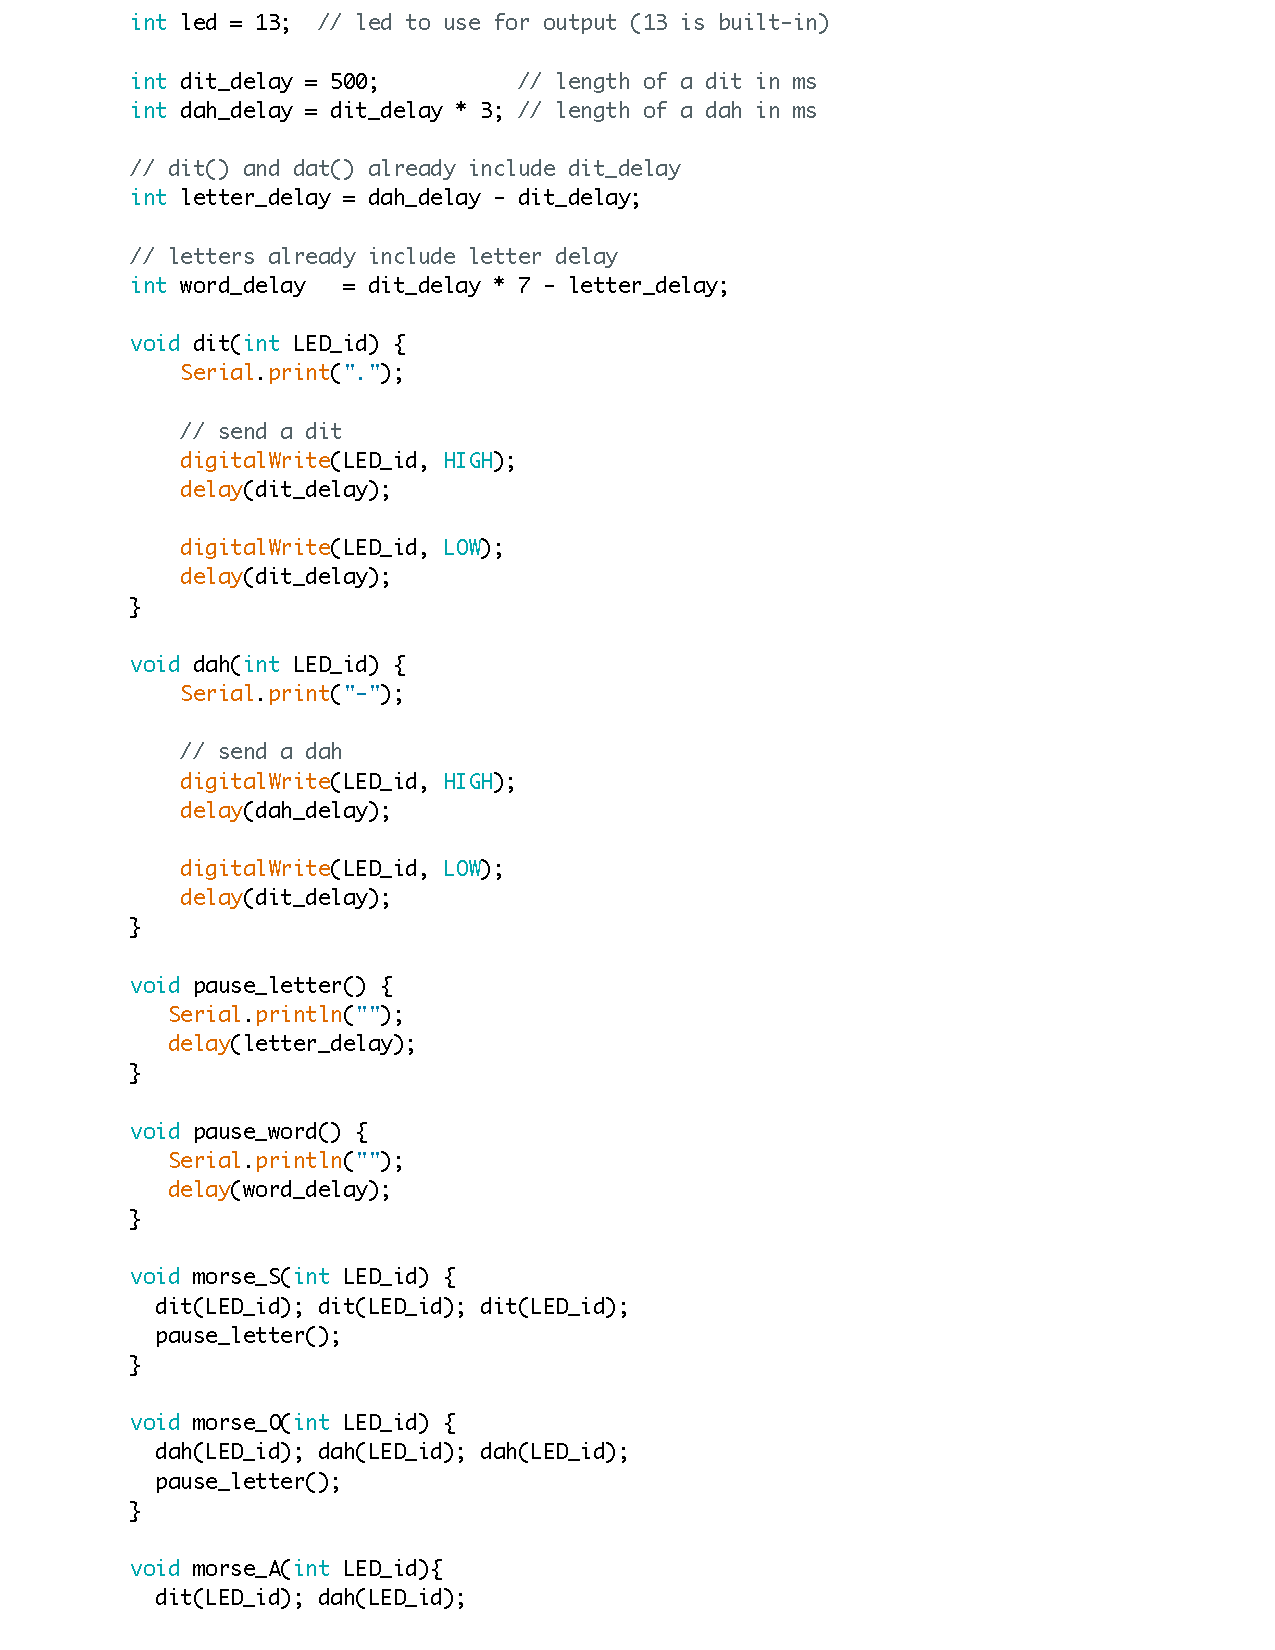
\includepdf[pages=-]{../aufgabe22/aufgabe22.pdf}

        now you can just call the function with the id of the LED you want the letter to appear as shown in the file for this task. You can replace the LED id 13 with any other LED if you would like!

    \item


\end{enumerate}


\end{document}
